

\documentclass[xetex,mathserif,serif]{beamer}
%\documentclass{beamer}
\usetheme{Madrid}
\usecolortheme{beaver}
\usepackage{textpos}
\usepackage{listings}
\usepackage{fontawesome}
\usepackage{fontspec}
\newfontfamily{\FA}{FontAwesome.otf}

\def\twitter{{\FA \faTwitter}}

\def\home{{\FA \faHome}}
\def\github{{\FA \faGithubSign}}


\title{D3.js meet ICU Patients}
\author[TWSS]{
\includegraphics[height=5cm,width=7cm, keepaspectratio,angle=270] {twss.pdf}\\That what she said.}
\institute[Team]{Marcin Tolysz and Geoff Hogg }
\date{\today}

\begin{document}

\begin{frame}
  \maketitle
\end{frame}

\addtobeamertemplate{frametitle}{}{%
 \begin{textblock*}{10mm}(.85\textwidth,-1cm)
 
\includegraphics[height=2cm,width=3cm, keepaspectratio,angle=270] {twss.pdf}
 %\includegraphics[height=1cm,width=2cm]{cat}
\end{textblock*}}

  \begin{frame}{Motivation}
    %\frametitle{Motivation}
   \begin{block}{Have fun}
      This is a primary motivator for the weekends
   \end{block}
   \pause
   \begin{block}{Learn something}
      This motivates my life
   \end{block}
   \pause
   \begin{alertblock}{Do something}
      This is a benchmark of how much we learned
   \end{alertblock}
   \pause
   \begin{exampleblock}{Win something}
      Sure, but not really.
   \end{exampleblock}
  \end{frame}
  \begin{frame}
    \frametitle{What did we do}
    \framesubtitle{The main steps}

   \begin{block}{Infrastructure}
      Set the server and config
   \end{block}
   \pause
   \begin{block}{Download Data}
      Decision of for the task to do.
   \end{block}
   \pause
   \begin{alertblock}{Visualising Data}
      We had a small team (2 people), so we had to choose something light.
   \end{alertblock}
  \end{frame}
  \begin{frame}
    \frametitle{ICU Patients}
    \framesubtitle{FIFO}
 
 \begin{columns}[T]
   \begin{column}{.6\textwidth}

   \begin{block}{Clean Data}
  \pause
      Haskell
   \end{block}
\pause
   \begin{alertblock}{plain text -> one big JSON}
  \pause
      D3js
   \end{alertblock}
 
      \end{column}
  \begin{column}{.4\textwidth}
  \pause
    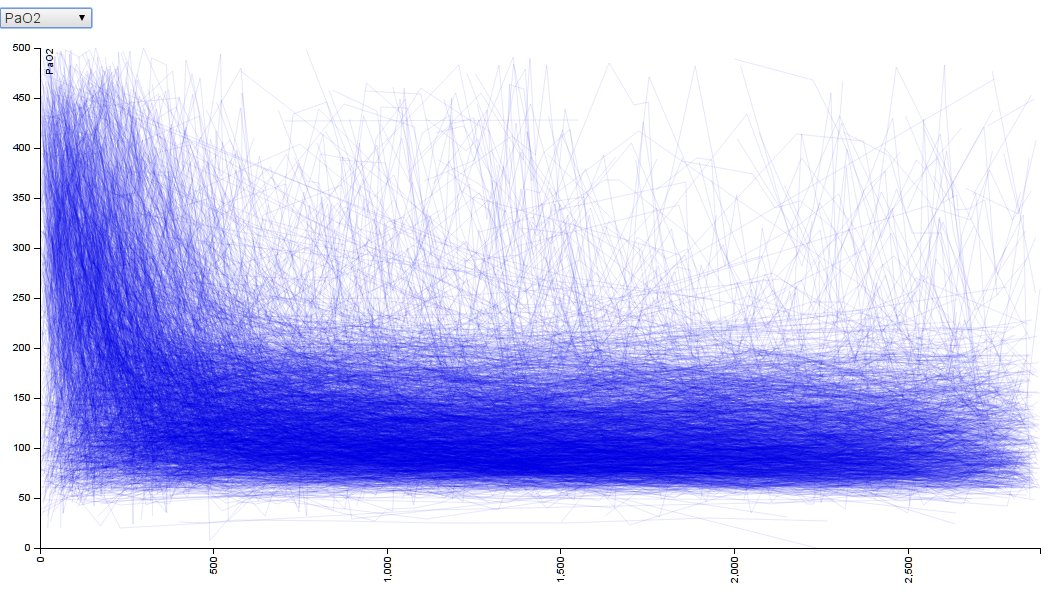
\includegraphics[height=5cm,width=7cm, keepaspectratio,angle=270] {PaO2.pdf}
 \end{column}
  \end{columns}

%  \pause
%   \begin{verbatim}
%       {"HCT":[{"time":188,"value":33.7}
%              ,{"time":637,"value":33.5}
%              ,{"time":1987,"value":30.3}
%              ]
%       ,"Height":[{"time":0,"value":-1}]
%       ,"HR":[{"time":7,"value":73}
%       ...
 %  \end{verbatim}
%   \pause
 %  \begin{block}{Download Data}
%      Decision of for the task to do.
 %  \end{block}
  \end{frame}

 \begin{frame}
    \frametitle{ICU Patients}
    \framesubtitle{The Last Slide}

\begin{columns}[T]
 \begin{column}{.4\textwidth}
   \includegraphics[height=5cm,width=7cm, keepaspectratio,angle=0] {slide.pdf}
 \end{column}
 \begin{column}{.6\textwidth}
\pause
   \begin{block}{Questions?}

     \href{https://twitter.com/mtolysz}{\twitter\  mtolysz} 
\pause

     \href{https://twitter.com/zeristor}{\twitter\  zeristor}
\pause

     \href{ https://twss.s5.tolysz.org/marcin/ }{\home\  https://twss.s5.tolysz.org/marcin/ }
\pause

     \href{ https://github.com/tolysz/ohdh14 }{\github\  https://github.com/tolysz/ohdh14 }
     
  \end{block}
 \end{column}
  \end{columns}
  \end{frame}
%

% etc
\end{document}